% !TEX root = ../main.tex
\chapter{Introduction to Spectroscopy}
\label{chapter_spectroscopy}
%-------------------------------------------------------------------------------
%	SECTION 1: INTRODUCTION TO SPECTROSCOPY
%-------------------------------------------------------------------------------


\todoimp{where to put this?
\noindent
This polarization can be decomposed into positive and negative frequency components. For the spectroscopic measurements the positive frequency part is relevant as the emitted signal field is proportional to it \todoref{IS THIS TRUE??} \cite{mukamel1995principlesnonlinearoptical}



This holds in the slowly varying amplitude approximation \cite{mukamel1995principlesnonlinearoptical}.

}

\noindent
\todoimp{find a better place for this

Now that we have seen the most general third order nonlinear optical processes, we will have to find a way to simplify the allowed interactions.

}



\section{Fundamentals of Spectroscopy}
\label{sec:spectroscopy_fundamentals}

\todoidea{This chapter	 should serve as a foundation by emphasizing electronic transitions, nonlinear optics, coherence phenomena, and their relevance to complex (e.g., biological) systems.
Vibrational and other spectroscopies are less relevant for this work, so they should be mentioned but not in detail.

Purpose: Set motivation and scope in two tight paragraphs.

What spectroscopy probes (energy levels → structure/dynamics).

Your scope: electronic spectroscopy, third-order nonlinear optics, 2DES. Mention that vibrational/rotational appear only as context.

One sentence on how this chapter supports later simulation sections.

}
\todoidea{
Brief motivation: Why spectroscopy is a powerful probe of quantum dynamics.

Distinction between linear and nonlinear optical spectroscopy.

Position of two-dimensional photon-echo spectroscopy (2D PES) within this landscape.

What this chapter provides: the physical and mathematical tools needed for later modeling.
}


\noindent 
Spectroscopy, in its broadest definition, is the study of the interaction between matter and electromagnetic radiation as a function of wavelength or frequency \cite{berman2011principleslaserspectroscopy, mukamel1995principlesnonlinearoptical}.
It provides insights into the composition, structure, and dynamics of physical systems by examining how they absorb, emit, or scatter light. The fundamental principle underlying all spectroscopic methods is that each atom, molecule, or complex system has a unique set of energy levels, and transitions between these levels involve the absorption or emission of photons with specific energies \todoref{find better source}\cite{boyd2008chapter1nonlinear}. Thats why spectroscopy is a powerful probe of quantum dynamics.



\subsection{Basic Principles}
\label{subsec:basic_principles}

\noindent The foundation of spectroscopy rests on the quantization of energy in atomic and molecular systems. According to quantum mechanics, atoms and molecules can exist only in discrete energy states \cite{albashetal2012quantumadiabaticmarkovian}. The energy difference between two such states, $\Delta E$, determines the frequency $\nu$ or wavelength $\lambda$ of light that can be absorbed or emitted during a transition between these states, following Planck's relation:

\begin{equation}
	\Delta E = h\nu = \frac{hc}{\lambda}
	\label{eq:planck_relation}
\end{equation}

\noindent
where $h$ is Planck's constant and $c$ is the speed of light. The energy structure of matter can thus be probed by observing the spectrum of absorbed or emitted radiation.

\noindent
To characterize the most common spectroscopic techniques, it is vital to understand the energy scales of the system of interest and the probing electromagnetic radiation, because they have to match in order to effectively pump transitions.
The fundamental kinematic relations for the electromagnetic propagation in vacuum are

\begin{equation}
	\omega = 2\pi\nu, \qquad |\vec{k}| = \frac{2\pi}{\lambda}, \qquad \lambda = \frac{c}{\nu} = \frac{2\pi c}{\omega}
	\label{eq:wavelength_frequency_relation}
\end{equation}

\noindent 
with $\nu$ the (cycle) frequency in hertz (Hz), $\lambda$ the wavelength. 
%In a material medium the phase velocity is $v_p = c/n(\nu)$ and $\lambda$ is replaced by $\lambda_n = v_p/\nu = \lambda/n(\nu)$, where $n(\nu)$ is the refractive index.

\noindent 
Note that the \emph{magnitude of the wavevector } $k = 2\pi/\lambda$ (units m$^{-1}$), shall not be confused with the \emph{(spectroscopic) wavenumber} $\tilde{\nu}$, defined as

\begin{equation}
	\tilde{\nu} = \frac{1}{\lambda} \quad [\mathrm{cm}^{-1}].
	\label{eq:wavenumber_definition}
\end{equation}

This quantity is commonly used in spectroscopy. % TODO why is it used? to avoid large powers of ten. 
Now to give a broad idea of where transitions that one would like to probe with spectroscopy lie, we can look at the typical energy scales.

\subsection{Classification of Spectroscopic Techniques}
\label{subsec:classification_techniques}

\todoidea{can I also include some figure illustrating this?}
\noindent
Spectroscopy can be categorized by (i) the nature of the transition (rotational, vibrational, electronic, nuclear), (ii) the number of photons involved (linear vs.\ nonlinear), and (iii) the detection scheme (absorption, emission, or scattering). 

\noindent
(i):

\noindent
Different types of transitions are probed at distinct regions of the electromagnetic spectrum, reflecting the corresponding energy and time scales and providing fundamentally different information about the system of interest. 

\noindent
Ultrafast laser development has enabled femtosecond and even attosecond spectroscopy, allowing real-time tracking of electron motion and energy flow in complex systems.

\noindent
For example, rotational transitions lie in the microwave region. Here molecular geometry is revealed through quantized rotational energy levels. In vibrational spectroscopy, bonding patterns are measured within the infrared ($\lambda\!\sim\!2.5$–$25\,\mu\mathrm{m}$, $\tilde{\nu}\!\sim\!400$–$4000\,\mathrm{cm^{-1}}$) region of the spectrum. In this thesis electronic transitions between molecular orbitals will be probed with visible frequencies of  ($\lambda\!\sim\!400$–$750\,\mathrm{nm}$, $\tilde{\nu}\!\sim\!13{,}000$–$25{,}000\,\mathrm{cm^{-1}}$), enabling studies of excited-state structure and dynamics.

\noindent
This energetic hierarchy underlies the classification of spectroscopic techniques: higher photon energies probe faster and more localized motions.
While timescales of Micro-milliseconds relate to  Chemical reactions and protein folding, Vibrational relaxation and rotational dynamics happen at picoseconds. Important for this thesis, electronic transitions and vibrational coherences occur at femtoseconds. Recent advances in attosecond spectroscopy now even allow probing real time electron dynamics within atoms and molecules \cite{rupprechtetal2025tracinglonglivedatomic}.

\subsection{Energy Dissipation After Absorption}

\noindent
After an interaction with the electromagnetic field, absorption of a photon, the excited molecule relax through two principal pathways:
\textbf{Non-radiative relaxation:} Internal conversion and vibrational energy transfer to the environment convert excitation energy into heat. What will be important for this thesis is \textbf{Radiative relaxation} where the ground state is populated again. In a experiment the emitted photons that are typically isotropic and thus contribute little to the forward beam.

\noindent
Absorption spectra thus record the net loss of intensity from the incident mode, while emission spectra provide complementary information on excited-state structure and relaxation dynamics. Both will be central in later sections involving heterodyne detection of emitted fields. \todoref{find ref and connect to later sections}



\subsection{Macroscopic Samples and Collective Dipolar Oscillations}
\label{subsec:macroscopic_samples}

\noindent 
When considering spectroscopic measurements on macroscopic samples, it is essential to understand how individual molecular responses combine to produce observable signals. In a typical spectroscopic experiment, the sample contains on the order of Avogadro's number ($\sim 10^{23}$) of molecules, each potentially acting as an oscillating electric dipole when interacting with electromagnetic radiation \cite{feynman1965feynmanlecturesphysics}.

\noindent 
The collective behavior of these molecular dipoles determines the induced macroscopic polarization of the sample. When an external electromagnetic field is applied, individual molecules undergo dipole transitions, creating time-varying dipole moments $\vec{\mu}_i(t)$. The coherent superposition of these individual dipolar oscillations produces a macroscopic polarization wave $\vec{P}(\vec{r}, t)$ that can be detected experimentally

\begin{equation}
	\vec{P}(\vec{r}, t) = \frac{1}{V} \sum_{i} \vec{\mu}_i(t) \delta(\vec{r} - \vec{r}_i).
	\label{eq:macroscopic_polarization}
\end{equation}

\noindent 
where $V$ is the sample volume, $\vec{r}_i$ is the position of the $i$-th molecule, and the sum extends over all molecules in the interaction region. This polarization acts as a source term in Maxwell's equations, generating the electromagnetic fields that constitute the spectroscopic signal \cite{abramaviciusetal2009coherentmultidimensionaloptical}

\begin{equation}
	\nabla \times \nabla \times \vec{E}(\vec{r}, t) + \frac{1}{c^2} \frac{\partial^2}{\partial t^2} \vec{E}(\vec{r}, t) = - \frac{4 \pi}{c^2} \frac{\partial^2}{\partial t^2} \vec{P}(\vec{r}, t).
\end{equation}

\noindent
A formal solution of the wave equation shows that the emitted polarization at position $\vec{r}$ and time $t$ is given by

\begin{equation} \label{eq:solution_wave_equation}
	\vec{P}_S(\vec{r}, t) = \vec{P}(t) \exp(i \vec{k}_S \cdot \vec{r} - i \omega_S t) + \text{c.c.}
\end{equation}

\noindent
where $\vec{k}_S$ and $\omega_S$ are the wavevector and frequency of the emitted signal, respectively. The connection to incident fields is essential for photon-echo and other nonlinear spectroscopies discussed later. 

\noindent 
In the slowly varying amplitude approximation, the emitted signal field $\vec{E}_S$ is directly proportional to the macroscopic polarization \cite{mukamel1995principlesnonlinearoptical}. This approximation holds when the magnitude of the polarization varies slowly compared to the optical cycle of the incident field. A short derivation can be found in \cite{boyd2008chapter6nonlinear}.
\todoidea{a bit more explanation (mathematical), page 295 complex polarization is mentioned!}

\begin{equation} \label{eq:signal_field_propto_P}
	\vec{E}_S(\vec{r}, t) \approx i \vec{P}_S(\vec{r}, t)
\end{equation}

\noindent 
\todoidea{add the following paragraph to a different section, but which?}
The phase relationships between individual dipolar oscillations are crucial for understanding spectroscopic line shapes and signal intensities

\noindent 
In the case of inhomogeneously broadened systems\footnote{\todoidea{ALSO ADD: When the harmonic potential surfaces of the ground and the excited states are dis
placed, the energy gap between the ground and the excited state will vary linearly
 with the nuclear coordinate q. A uctuating coordinate due to thermal excitation of
 the nuclear coordinates hence will give rise to a uctuating transition frequency. In
 that sense the Brownian oscillator model is a more microscopic model, which speci¯es
 the reason for a uctuating transition frequency \cite{hamm2005principlesnonlinearoptical} page 58
}}, different molecules oscillate at slightly different frequencies due to variations in their local environment. The resulting dephasing of individual oscillators leads to the characteristic decay of macroscopic coherences observed in techniques such as photon echo spectroscopy \cite{mukamel1995principlesnonlinearoptical}.


\todoidea{Figure out how to connect the next to later sections.

This was an earlier version, but I don't like it anymore:
The standard way to calculate the nonlinear response is to use response function formalism, which will be discussed in the next section.
}
\section{Light-matter interaction - Calculation of the Polarization}
\label{sec:light_matter_interaction}

\noindent
The startpoint will be the semiclassical Hamiltonian of a quantum mechanically modeled matter-system interacting with classical radiation field described with vector and scalar potentials

\begin{equation}
	H = \frac{1}{2m} [\mathbf{p} + q \mathbf{A}(\mathbf{r}, t)]^2 + V(\mathbf{r}) - q \phi(\mathbf{r}, t)
	\label{eq:hamiltonian}
\end{equation}

\noindent
where $\mathbf{p}$ is the momentum operator, $q$ the electric charge of the system, $V(\mathbf{r})$ the potential energy of the matter system, $\mathbf{A}(\mathbf{r}, t)$ the vector potential, and $\phi(\mathbf{r}, t)$ the scalar potential of the electromagnetic field \cite{cohen-tannoudjietal2008atomphotoninteractionsbasic}. Standard procedure is to go into the dipole approximation, meaning the spatial variation of the field over the extent of the molecule is negligible, and the Coulomb gauge, where $\nabla \cdot \mathbf{A} = 0$ and $\phi = 0$, to simplify the Hamiltonian to the commonly used form \todoref{find ref}
In this case, the Hamiltonian takes the form

\begin{equation}
	H = H_0 + V(t).
\end{equation}

\noindent 
where $H_0$ is the unperturbed Hamiltonian of the matter system and the interaction term is given by

\begin{equation} \label{eq:dipole_approx_term}
	V(t) = - \mathbf{\hat{\mu}} \cdot \mathbf{E}(t).
\end{equation}

\noindent
where $\mathbf{E}(t)$ is the electric field and $\mathbf{\hat{\mu}}$ is the dipole operator of the matter system. 
This allows us to calculate the macroscopic polarization as the expectation value of the microscopic dipole operator (see Eq. \eqref{eq:ho_expectation_value})

\begin{equation}
	\vec{P}(t) = \langle \mathbf{\hat{\mu}}(t) \rangle = \mathrm{Tr}[\mathbf{\hat{\mu}} \rho(t)]
	\label{eq:polarization_expectation_value}
\end{equation}


\noindent
Now that we have introduced the most important quantity in spectroscopy Eq. \ref{eq:macroscopic_polarization}, and found out how to calculate it in the previous section, we can discuss how it depends on the incident electric field. This leads to nonlinear optics.

%----------------------------------------------------------------------------------------
%	SECTION 2: NONLINEAR OPTICS
%----------------------------------------------------------------------------------------
\section{Nonlinear Optics}
\label{sec:nonlinear_optics}
\todoidea{typically at high field intensities, the response of the medium becomes nonlinear.}
\todoidea{explain Response theory as the standard way to deal with this -> it is a perturbative approach -> mine is numerical and better cite leszczynskietal2017handbookcomputationalchemistry, the most modern one is loaizaetal2025nonlinearspectroscopygeneralized}


In general, the polarization can be expanded as a power series in the incident electric field:
\todoimp{clarify the tensor component of this quantity}

\begin{equation}
	\vec{P} = \varepsilon_0 (\chi^{(1)} \vec{E} + \chi^{(2)} \vec{E} \cdot \vec{E} + \chi^{(3)} \vec{E} \cdot \vec{E} \cdot \vec{E} + \ldots)
	\label{eq:nonlinear_polarization}
\end{equation}

\noindent 
where $\varepsilon_0$ is the vacuum permittivity and $\chi^{(i)}$ is the $i$-th-order nonlinear susceptibility tensors.  This is going to be usefull for interpreting numerically exact (but with not clearly separated pathways) results later on.

\noindent 
In the linear regime, the induced polarization $\vec{P}$ can be cut after the first contribution, which is directly proportional to the applied electric field $\vec{E}$.
This relationship describes phenomena such as refraction and absorption.
The higher-order terms give rise to a variety of nonlinear optical phenomena \cite{boyd2008contents}.

\noindent 
\todoidea{leave it out completely?}
Second-order nonlinear processes are not important for this thesis, but mentioned for completeness.
They are governed by the $\chi^{(2)}$ term and occur only in noncentrosymmetric materials, which lack inversion symmetry \cite{rao2018overviewsecondthird,boyd2008chapter1nonlinear}.  Second-order nonlinear processes include Second Harmonic Generation (SHG), where two photons of frequency $\omega$ combine to generate a photon of frequency $2\omega$; Sum Frequency Generation (SFG), where two photons of frequencies $\omega_1$ and $\omega_2$ combine to produce a photon of frequency $\omega_1 + \omega_2$; Difference Frequency Generation (DFG), where two photons interact to create a photon of frequency $\omega_1 - \omega_2$.

\noindent
Already in the second-order nonlinear processes, the new rich phenomena appear compared to linear optics.
Now we can move on to the third-order nonlinear processes, which powers two dimensional spectroscopy and thus are the main focus of this thesis.



\subsection{Third-Order Nonlinear Processes}
\label{subsec:third_order}
\todoidea{change the order of phase matching <-> third order nonlinear process}
\todoidea{Add intuition for what the pulse phase kick does for delta pulses -> visual representation on bloch sphere like in \cite{grolletal2025fundamentalsheterodynewave} also the pulse area!! }
\noindent
We write the electric field that couples to the system via Eq. \eqref{eq:dipole_approx_term} as 

\begin{equation} \label{eq:electric_field_three_pulses}
E(t)=\sum_{a=1}^3 E_a e^{i \vec{k}_a \cdot \vec{r} - i\omega_a t} + \text{c.c.}
\end{equation}

\noindent
and use the analytic–conjugate split $E^{(+)}(t)$, $E^{(-)}(t)=[E^{(+)}(t)]^*$. Then the third order component of the polarization Eq. \eqref{eq:nonlinear_polarization} is given by

\begin{equation}
P_i^{(3)}(t)
=\varepsilon_0 \sum_{jkl}\sum_{\sigma_1,\sigma_2,\sigma_3=\pm 1}
\chi^{(3)}_{ijkl}(-\omega_S;\sigma_1\omega_1,\sigma_2\omega_2,\sigma_3\omega_3)\,
E_j^{(\sigma_1)}E_k^{(\sigma_2)}E_l^{(\sigma_3)}\,e^{-i\omega_S t},
\end{equation}

\noindent
with $\omega_S=\sigma_1\omega_1+\sigma_2\omega_2+\sigma_3\omega_3$.
This means already the interacting field contains $6 \times 6 \times 6 = 216$ terms, with the following $22$ unique positive frequencies (grouping by $\omega_S>0$ yields the distinct components):

\begin{equation} \label{eq:general_third_order_freqs}
\{\omega_i\},\ \{3\omega_i\},\ \{2\omega_i\pm\omega_j\}_{i\neq j},\ 
\{\omega_1+\omega_2+\omega_3\},\ \{\omega_i+\omega_j-\omega_k\}_{i\neq j\neq k}.
\end{equation}

\noindent
Third-order, nonlinear processes can occur in all materials, regardless of symmetry \cite{hamm2005principlesnonlinearoptical}. 
\todoimp{the following is not really relevant; IF include, find better connection to earlier \& later stuff}
Key third-order nonlinear processes include Third Harmonic Generation (THG), where three photons combine to generate a photon of tripled frequency; Nonlinear Refraction, where the refractive index depends on light intensity, known as the Kerr effect; and Two-Photon Absorption (TPA), which involves the simultaneous absorption of two photons to excite a transition.

\noindent
However, the most important third-order process for this thesis is Four-Wave Mixing (FWM) \cite{boyd2008chapter6nonlinear}. Here, three incident and one generated photon interact in a way that satisfies energy conservation.
This process generates multiple possible pathways, including photon echo signals and allowing for 2D spectroscopy. This will be discussed in detail in the following sections. 


\noindent
First it would be helpful to isolate the effect of just one non-linear process theoretically, i.e. before being able to interpret experimental data. 
This will lead us to the framework of response functions in the following Sec. \ref{sec:response_functions}. Afterwords it will be possible to connect specific pathways to experimental observables via phase matching conditions in Sec. \ref{sec:phase_matching}.

\section{Response Functions}
\label{sec:response_functions}
In general, one can write Eq. \eqref{eq:polarization_expectation_value} in a perturbative series expansion

\begin{equation}
	\vec{P}(t) = \sum_n \vec{P}^{(n)}(t) = \sum_n \langle \mathbf{\hat{\mu}}(t) \rangle = \mathrm{Tr}[\mathbf{\hat{\mu}} \rho^{(n)}(t)],
	\label{eq:polarization_expectation_value_perturbative}
\end{equation}

\noindent
where only the quantity $\vec{P}^{(n)}(t)$ for a specific order of interest has to be calculated. Note that we are specifically interested in the third-order polarization $\vec{P}^{(3)}(t)$ for FWM processes, but the framework is kept general for now.

\noindent
The following equations are taken for the optical case of taking the dipole operator as the observable $A = \hat{\mu}$, with the dipole approximation Hamiltonian (Eq. \eqref{eq:dipole_approx_term}), but generally they hold for other observable as well, just producing different expectation values. \todoref{<- find examples?}
The $i$-th order polarization can be written as the convolution of $i$ electric fields \cite{hamm2005principlesnonlinearoptical}

\begin{align}
	P^{(i)}(t) &= \int_{0}^{\infty}\! dt_{i} \int_{0}^{\infty}\! dt_{i-1} \cdots \int_{0}^{\infty}\! dt_{1} \notag \\
	&\quad E\bigl(t-t_{i}\bigr)\, E\bigl(t-t_{i}-t_{i-1}\bigr)\,\cdots\, E\bigl(t-t_{i}-\cdots - t_{1}\bigr) \notag \\
	&\quad R(t_{i},t_{i-1},\ldots,t_{1}),
	\label{eq:response_convolution}
\end{align}

\noindent
where the $i$-th response function is defined as

\begin{equation}
	R^{(i)}(t_{i},\ldots,t_{1})
	\;=\;
	\left(-\frac{i}{\hbar}\right)^{i}
	\Big\langle
	\hat{\mu}(t_{i}+\cdots + t_{1})\;[\hat{\mu}(t_{i-1}+\cdots + t_{1}),\ldots [\hat{\mu}(0),\rho(-\infty)]\ldots]
	\Big\rangle
	\label{eq:response_function_R}
\end{equation}

\noindent
and describes the system's response to $i$ interactions with the electric field.
Here $\hat{\mu}(t)$ is the dipole operator in the interaction picture.
Note, that the interactions at the different times $t - t_{i} - \ldots$ can occur in any order.
Also note, that the response function only depends on the material under investigation \cite{hamm2005principlesnonlinearoptical}.
It is assumed that the interaction takes place at local times $t_i$ (short pulse limit), and the system is in an equilibrium state (the ground state) before the interaction, at time $t = - \infty$.
It is crucial that the first $i-1$ dipole operators are inside nested commutators, that represent how these field-interactions drive the system out of equilibrium. The last operator then represents the emitted field and is measured by being traced over the environmental degrees of freedom.
Explicitly, the commutators in Eq-\eqref{eq:response_function_R} contains $2^i$ terms with multiple actions of $\hat{\mu}$ on the left / right on the density matrix.
Thought one can ignore the complex conjugate contributions, reducing to $2^{i-1}$ terms.
Each such term corresponds to a specific sequence of field interactions and can be represented with double-sided Feynman diagrams \cite{mukamel1995principlesnonlinearoptical}. In it the left and right sides of the diagram represent the evolution of the ket and bra states of the density matrix, respectively. Each interaction with the electric field is depicted as an arrow, with arrows pointing towards the density matrix indicating absorption (interaction from the left) and arrows pointing away indicating emission (interaction from the right). The time intervals between interactions are represented by horizontal lines, during which the system evolves freely according to its Hamiltonian.
\todoidea{add a example figure for the simplest linear polarizataion and then later the pathways for the third order response function.}


\noindent
Eq. \eqref{eq:response_convolution} is the central equation in two dimensional spectroscopy \cite{segarra-martietal2018accuratesimulationtwodimensional}. Each experimentally observed signal direction (phase matched condition Eq. \eqref{eq:phase_matching}) isolates a subset of the possible Liouville-space pathways of the system.
Accordingly, the total response in that direction can be written as a sum over all contributing pathways,
\begin{equation}
	R^{(i)}(t) = \sum_{\text{path}} R_{\text{path}}(t),
	\label{eq:Liouville_pathways}
\end{equation}
where $R_{\text{path}}(t)$ represents the contribution of a single Liouville pathway corresponding to a specific sequence of field interactions and density-matrix evolutions.


\noindent
As mentioned in Sec \ref{subsec:third_order}, FWM is the method discussed in detail. It is a third-order process, so $i=3$ in Eq. \eqref{eq:response_convolution} and \eqref{eq:response_function_R}. The response function can be separated into different contributions, depending on the time ordering of the three field interactions. This leads to four main contributions, which can be represented with double-sided Feynman diagrams \cite{mukamel1995principlesnonlinearoptical}.


The setup can be seen in Fig. \ref{fig:fwm_box_car_setup}. Here three pulses with wavevectors $\mathbf{k}_1, \mathbf{k}_2, \mathbf{k}_3$ interact with the sample and generate a signal in the direction $\mathbf{k}_S$. 

\noindent
This thesis will instead use a more microscopic non-perturbative (NP) approach.
Here first the total signal will be calculated, where all pulses are active, and then the desired order will be extracted by filtering out the linear contributions, where only the $i$-th pulse is active.
This way the third order signal can be calculated by 

\begin{equation}
	P^{(3)}(t) = P_{\text{total}}(t) - P_{(2)}(t) - P_{(1)}(t) - P_{(0)}(t)
	\label{eq:third_order_signal_numerical}
\end{equation}

\noindent
where the Polarization from Eq. \eqref{eq:polarization_expectation_value} is used. \todofix{actually not true as only the analytical component is extracted, to include phase information.}



% TODO uncomment these figures
\todofix{uncomment figures (for git -> also include svgs?)}
\begin{figure}[ht]
	\centering
	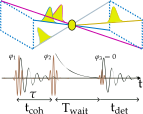
\includegraphics[width=0.8\textwidth]{../figures/FWM_scheme.pdf}
	\caption{Schematic Four-wave mixing setup in a Boxcar geometry. ... \todoimp{Add description. Add S, Add wavevectors, Reduce amplitude of probe pulse.}}
	\label{fig:fwm_box_car_setup}
\end{figure}

\begin{figure}[ht]
	\centering
	\includegraphics[width=0.8\textwidth]{../figures/FWM_scheme_phase_cycling.pdf}
	\caption{Schematic Four-wave mixing setup. This is the simpler collinear phase-cycling setup, at the cost of requiring multiple measurements with varied pulse phases.
	\todoidea{add ground state at beginning, }}
	\label{fig:fwm_phase_cycling_setup}
\end{figure}

\todoidea{Interaction picture, (introduce but defer justification).}
\todoidea{Also include how to simulate laser pulses:
Gaussian envelope, pulse trains.
1) Time-domain field (carrier × envelope)
$f(t)$ = envelope (e.g. Gaussian $f(t) = \exp\left[-\frac{2\ln 2}{\tau_{\mathrm{FWHM}}^2} t^2\right]$),

$\phi_{\mathrm{CE}}$ = carrier--envelope phase (relevant for few-cycle pulses),

$E_0$ sets peak field (related to pulse energy via the mode area and duration).

Bandwidth for a transform-limited Gaussian:

$\Delta\omega_{\mathrm{FWHM}} \approx \frac{2\ln 2}{\tau_{\mathrm{FWHM}}}$}


%-------------------------------------------------------------------------------
%   NEW SUBSECTION: CHARACTERIZATION OF ELECTROMAGNETIC RADIATION
%-------------------------------------------------------------------------------
\subsection{Characterization of Electromagnetic Radiation}
\label{subsec:em_radiation_characterization}
\todoimp{this section is NOT needed here}

\noindent 
A monochromatic electromagnetic plane-wave in free space (vacuum) can be written as

\begin{equation}
	E(\vec{r},t) = E_0 \cos(\vec{k} \cdot \vec{r} - \omega t + \phi)
	\label{eq:plane_wave}
\end{equation}

\noindent 
where $E_0$ is the (real) amplitude, $\phi$ a phase-kick, $\vec{k}$ the wavevector (spatial angular frequency), and $\omega$ the angular frequency of the wave. The real field can be decomposed into complex positive and negative frequency parts as

\iffalse
\begin{equation}
	E^{(+)} = E_0 e^{i(\vec{k} \cdot \vec{r} - \omega t + \phi)}
	\label{eq:positive_frequency_e_field}
\end{equation}

\noindent 
with $E^{(-)} = E^{(+)}^{*}$ and thus $E = 1/2 \{E^{(+)} + E^{(-)}\}$.
$E^{(+)}$ is called the positive-frequency part because in Fourier space it contains only components with frequencies $\omega > 0$ \todoref{fact check}. This will come in handy applying a rotating wave approximation as the positive field part rotates in the same direction as the rotating frame and the negative rotates in the opposite direction \cite{hamm2005principlesnonlinearoptical}.
\fi





\section{Wavevector Phase-Matching Conditions}
\label{sec:phase_matching}

\noindent 
In nonlinear optical processes, multiple light waves interact within a material to generate new frequencies. Like mentioned before, momentum conservation of the incident and outgoing photons has to be met. For a general third order nonlinear process, the wavevector of the generated signal ($\vec{k}_S$) is determined by the vector sum of the input wavevectors:

\begin{equation}
	\vec{k}_S = \pm\vec{k}_1 \pm\vec{k}_2 \pm\vec{k}_3.
	\label{eq:four_wave_mixing}
\end{equation}

\noindent
This is called the phase-matching condition.
The signs depend on whether the corresponding field acts on the ket or bra branch of the density matrix: absorption (ket interaction) contributes $+\vec{k}_i$, while emission or complex-conjugate interactions (bra side) contribute $-\vec{k}_i$. 
A drastic simplification (reduction of the terms in \eqref{eq:general_third_order_freqs}) transforming into a frame that rotates with the optical field. In this rotating-wave approximation (RWA) the positive-frequency component of the field $E_i(t) \propto e^{-i\omega_i t}$ couples via the lowering dipole $\hat{\mu}_{-}$ to the ket, and the complex-conjugate component $E_i^{*}(t) \propto e^{+i\omega_i t}$ couples via $\hat{\mu}_{+}$ to the bra. Consequently, the sign in Eq.~\eqref{eq:four_wave_mixing} tracks which side of the density matrix the field interacted with.

\noindent
Different combinations of signs correspond to different phase-matching conditions, leading to signals in different spatial directions. These distinct signal directions allow separation of various nonlinear optical processes. The two most important phase-matching conditions for this thesis are presented in the following.



\subsection{Rephasing and nonrephasing Signals}
\label{subsec:rephasing_nonrephasing}

\noindent
To further reduce the number of contributions to the third-order polarization (alongside RWA), one can enforce strict time ordering of the pulses (impulsive limit, where there are no overlap of the well separated delta pulses \cite{cho2009twodimensionalopticalspectroscopy, hamm2005principlesnonlinearoptical}).

Now the the only surviving terms in the third order polarization are the so called \textit{rephasing} and \textit{nonrephasing} contributions \cite{cho2009twodimensionalopticalspectroscopy, jonas2003twodimensionalfemtosecondspectroscopy}.
\textbf{Rephasing signal} follow the phase-matching condition $\vec{k}_S = -\vec{k}_1 + \vec{k}_2 + \vec{k}_3$. The sign pattern now reads directly as the interaction sequence: ($-\vec{k}_1$) the first pulse acts from the bra side, ($+\vec{k}_2$) the second pulse acts from the ket side, and ($+\vec{k}_3$) the third pulse again acts from the ket side. Diagrammatically this reproduces the arrow directions in Fig.~\ref{fig:fwm_phase_cycling_setup}. The first interaction creates a coherent superposition between ground and excited states, generated by a complex conjugate interaction of the bra. The second pulse converts this coherence into a population, and the third pulse generates a new coherence that emits the signal. The phase accumulated due to different frequencies can be reversed during the period between the third interaction and signal emission. This leads to a photon echo effect at $t_{\text{det}} \approx t_{\text{coh}}$ where the dephased components rephase.
This happens for an inhomogeneously broadened ensemble of systems, where different realizations of the system have different transition energies, while the laser pulses drive at constant frequency of $\omega_L$. As a result, some realizations dephase quicker than others. Some realizations should come back in phase around $t_{\text{det}} \approx t_{\text{coh}}$ which is exactly this photon echo.
Contrary to this, \textbf{nonrephasing signal} satisfy $\vec{k}_S = +\vec{k}_1 - \vec{k}_2 + \vec{k}_3$. The field ordering is now: ($+\vec{k}_1$) first interaction on the ket (absorption), ($-\vec{k}_2$) second interaction on the bra (emission-like), and ($+\vec{k}_3$) third interaction on the ket. The first pulse therefore creates a forward-evolving coherence, the second pulse transfers it to the opposite branch, and the phase evolution at the third pulse continues in the same direction such that no echo is formed.


\subsection{Phase Cycling in Nonlinear Spectroscopy}
\label{subsec:phase_cycling}

\noindent 
While phase-matching enables the spatial isolation of desired nonlinear Liouville pathways, phase cycling provides an alternative approach by distinguishing signals based on their phases rather than their spatial propagation directions. \todoref{find ref}%\cite{tan2008, yan2009}.
\cite{mukamel1995principlesnonlinearoptical, cho2009twodimensionalopticalspectroscopy, jonas2003twodimensionalfemtosecondspectroscopy, brixneretal2004phasestabilizedtwodimensionalelectronic, greenetal2024vibrationalcoherenceshalfbroadband}.

\noindent 
Here the collinear beam line geometry can be used, simplifying the experimental setup.
This technique is particularly valuable when studying samples without scattering.

\noindent 
And for simulations, as done here, it facilitates the separation of rephasing and nonrephasing signals within the same measurement series.

\noindent 
In phase cycling, multiple measurements are taken with systematically varied phases of the excitation pulses. The desired nonlinear signals can then be extracted through appropriate linear combinations of these measurements. The fundamental principle relies on the fact that different nonlinear pathways respond distinctly to changes in the phases of the input fields.

\noindent 
For a third-order signal generated by three excitation pulses with phases $\phi_1$, $\phi_2$, and $\phi_3$, as seen in Fig. \ref{fig:fwm_phase_cycling_setup}.

\noindent 
By varying the input phases through a complete cycle (in steps of $\pi/2$) and applying discrete Fourier transform to the collected data, specific pathways can be isolated based on their phase dependencies.


\subsection{Phase-Cycling Fourier Selection and Construction of 2D Spectra}
\label{subsec:phase_cycling_fourier_selection}


\noindent 
The nonlinear polarization induced by three incident pulses can be expressed as a Fourier series in the pulse phases $\phi_1, \phi_2, \phi_3$, and individual phase-matched components are isolated via an inverse Fourier transform:

\begin{align}
	P^{(3)}_{n_1,n_2,n_3}(t_{\text{coh}},T,t_{\text{det}}) =
	\frac{1}{(2\pi)^3} \int_{0}^{2\pi}	\int_{0}^{2\pi} \int_{0}^{2\pi}  
	& d\phi_1 d\phi_2 d\phi_3
	e^{-i(n_1\phi_1+n_2\phi_2+n_3\phi_3)} \\
	& P^{(3)}(\phi_1,\phi_2,\phi_3;t_{\text{coh}},T,t_{\text{det}}).
	\label{eq:continuous_phase_cycling}
\end{align}

\noindent 
The physically relevant phase-matching directions correspond to:

\begin{align}
	\vec{k}_{\mathrm{R}}  & = -\vec{k}_1 + \vec{k}_2 + \vec{k}_3,
	                      & (n_1,n_2,n_3)                         & = (-1,+1,+1), \label{eq:rephasing_selection}    \\
	\vec{k}_{\mathrm{NR}} & = +\vec{k}_1 - \vec{k}_2 + \vec{k}_3,
	                      & (n_1,n_2,n_3)                         & = (+1,-1,+1), \label{eq:nonrephasing_selection}
\end{align}

\noindent 
yielding the rephasing (R) and nonrephasing (NR) contributions, respectively.

\noindent 
The (wavevector) phase-matched rephasing signal direction corresponds to selecting the Fourier index triple $(n_1,n_2,n_3)=(-1,+1,+1)$, while the nonrephasing direction corresponds to $(+1,-1,+1)$ \cite{mukamel1995principlesnonlinearoptical, cho2009twodimensionalopticalspectroscopy, greenetal2024vibrationalcoherenceshalfbroadband}.

\noindent 
The emitted field in a given phase-matching direction is proportional to the corresponding polarization\cite{jonas2003twodimensionalfemtosecondspectroscopy}:

\begin{equation}
	E_{k_s}(t_{\text{coh}},T,t_{\text{det}}) \propto i P_{\vec{k}_S}(t_{\text{coh}},T,t_{\text{det}}).
	\label{eq:field_polarization_relation}
\end{equation}

This holds in the slowly varying amplitude approximation \cite{mukamel1995principlesnonlinearoptical}.


\paragraph{Time--Frequency Transforms.}

\noindent 
So again i want to emphasize that first, dime domain signals of the third order polarization are calculated using Eq. \eqref{eq:polarization_expectation_value}, Eq. \eqref{eq:third_order_signal_numerical} and then the desired phase-matched contributions are extracted using Eq. \eqref{eq:continuous_phase_cycling}. 
After phase selection, the third order complex time-domain field $E_{k_S}(t_{\text{coh}}, T, t_{\text{det}})$ is Fourier transformed over the detection time $t_{\text{det}}$ and the coherence time $t_{\text{coh}}$ to construct the two-dimensional spectra \todoref{where is the eq?}%(cf. Eq.~\eqref{eq:2des_signal}):

\begin{align}
	S_{R}(\omega_{\text{coh}}, T, \omega_{\text{det}})
	 & =
	\int dt_{\text{coh}} \int dt_{\text{det}} \;
	e^{+ i \omega_{\text{coh}} t_{\text{coh}}} e^{- i \omega_{\text{det}} t_{\text{det}}}
	E_{R}(t_{\text{coh}}, T, t_{\text{det}}),
	\label{eq:rephasing_transform} \\
	S_{NR}(\omega_{\text{coh}}, T, \omega_{\text{det}})
	 & =
	\int dt_{\text{coh}} \int dt_{\text{det}} \;
	e^{- i \omega_{\text{coh}} t_{\text{coh}}} e^{- i \omega_{\text{det}} t_{\text{det}}}
	E_{NR}(t_{\text{coh}}, T, t_{\text{det}}).
	\label{eq:nonrephasing_transform}
\end{align}

\noindent 
The opposite sign in the $t_{\text{coh}}$-exponent implements the standard convention distinguishing rephasing (photon-echo) and nonrephasing contributions \cite{cho2009twodimensionalopticalspectroscopy, greenetal2024vibrationalcoherenceshalfbroadband}. In discrete numerical implementations, Eqs.~\eqref{eq:rephasing_transform}--\eqref{eq:nonrephasing_transform} are approximated by (shifted) fast Fourier transforms \cite{cho2009twodimensionalopticalspectroscopy, greenetal2024vibrationalcoherenceshalfbroadband}.

\paragraph{Absorptive Combination.}

\noindent 
The experimentally measured (or simulated) complex spectra $S_{R}$ and $S_{NR}$ can be combined to  construct the purely absorptive 2D spectrum \cite{mukamel1995principlesnonlinearoptical, jonas2003twodimensionalfemtosecondspectroscopy, greenetal2024vibrationalcoherenceshalfbroadband}
\begin{equation}
	S_{\text{abs}}(\omega_{\text{coh}}, T, \omega_{\text{det}})
	=
	\Re \left\{
	S_{R}(\omega_{\text{coh}}, T, \omega_{\text{det}}) + S_{NR}(\omega_{\text{coh}}, T, \omega_{\text{det}})
	\right\}.
	\label{eq:absorptive_spectrum}
\end{equation}

\noindent 
The absorptive spectra is free from broadening refractive contributions \cite{fullerogilvie2015experimentalimplementationstwodimensional}.



%----------------------------------------------------------------------------------------
%	SECTION 4: PHOTON ECHO SPECTROSCOPY
%----------------------------------------------------------------------------------------


\section{Heterodyne and Homodyne Detection Schemes}
\label{sec:heterodyne_homodyne}

\noindent Experimentally there are two main detection schemes used, influencing sensitivity and the information content of the measurements: homodyne and heterodyne detection \cite{abramaviciusetal2009coherentmultidimensionaloptical}.

\noindent
Generally the signal that arrives at the detector is proportional to the intensity of the emitted electric field, which is then integrated over a period of time by the detector

\begin{equation}
	S_{\text{det}} \propto \int I_{\text{det}}(t) \, dt.
	\label{eq:signal_intensity}
\end{equation}

\noindent On the one hand in homodyne detection, the intensity of the emitted signal field is measured directly, so $ I_{\text{HOD}} \propto |E_{\text{S}}|^2 \propto |P^{(3)}|^2 $. While experimentally simpler, homodyne detection loses phase information and it is more susceptible to noise at low signal levels \todoref{find ref or delete}%\cite{abramaviciusetal2009coherentmultidimensionaloptical}.

\noindent On the other hand, heterodyne detection involves the interference of the signal field with a reference field, the so called local oscillator (LO) of known amplitude and phase:

\begin{equation}
	I_{\text{HET}} \propto |E_{\text{S}} + E_{\text{LO}}|^2 \approx 2\Re{(E_{\text{LO}}^*E_{\text{S}})} + |E_{\text{LO}}|^2 + |E_{\text{S}}|^2
	\label{eq:heterodyne}
\end{equation}

\noindent Since $|E_{\text{LO}}| \gg |E_{\text{S}}|$, the cross-term dominates, and the signal can be extracted by phase-cycling. In contrast to homodyne detection, the heterodyned signal is not background-free but sits on an offset $\int E_{\text{LO}}(t)^2 \, dt$ which can be subtracted. Ideally, shaped pulses are used for the three input pulses and the local oscillator, yielding the response function directly: $\int E_{\text{LO}}(t) P^{(3)}(t) \, dt = S^{(3)}(t_3, t_2, t_1)$, without convolution complications, where $t_1$, $t_2$, $t_3$ are the directly controlled delays. This is exactly the analytically defined third-order response function in Eq. \eqref{eq:response_function_R}, making experimental data and simulations directly interpretable. This is the main strength of heterodyne detection \cite{mukamel1995principlesnonlinearoptical}. Also, it provides both amplitude and phase information of the signal. The signal scales linearly with the third-order response \todoref{find ref} \todoidea{why is this good?}

\noindent In modern multidimensional spectroscopy, spectral interferometry—a form of heterodyne detection—is widely employed \cite{hybletal1998twodimensionalelectronicspectroscopy}. The signal field and a time-delayed reference pulse are spatially overlapped and spectrally resolved.



\section{Photon Echo Spectroscopy}
\label{sec:photon_echo}
\noindent 
The echo intensity as a function of the delay time $t_{\text{coh}}$ reveals information about the dephasing processes in the system.

\noindent 
It is important to emphasize that static inhomogeneity is crucial for the appearance of the photon echo signal. This inhomogeneity arises from variations in the local environment of individual quantum systems within the ensemble, leading to a distribution of transition frequencies. In this thesis, in the numerical simulations, static inhomogeneity is taken into account by averaging the results over an ensemble of different realizations of the Hamiltonian \cite{cho2009twodimensionalopticalspectroscopy, mukamel1995principlesnonlinearoptical}. Without this inhomogeneous distribution, all systems would evolve identically, and the characteristic echo phenomenon would not occur.

\noindent 
By scanning the waiting time $T$, this technique allows measurement of population dynamics and spectral diffusion processes.

\subsection{Two-Dimensional Electronic Spectroscopy}
\label{subsec:2d_spectroscopy}

\noindent 
It correlates excitation and detection frequencies, revealing couplings between different transitions and energy transfer pathways.

\noindent 
Recall that a complete 2D spectrum is built from repeated three-pulse sequences while the coherence time $t_{\text{coh}}$ is scanned. The rephasing photon-echo signal arises after a finite rephasing time $t$ for sequences in which pulse 1 precedes pulse 2 ($t_{\text{coh}}>0$) and is recorded in the phase-matched direction $-\vec{k}_1 + \vec{k}_2 + \vec{k}_3$. As discussed in Subsec.~\ref{subsec:rephasing_nonrephasing}, the ground–excited coherences during $t_{\text{coh}}$ and $t$ accumulate opposite phases in the rephasing branch. When the ordering of pulses 1 and 2 is reversed ($t_{\text{coh}}<0$), these phase factors add rather than cancel, yielding a nonrephasing free-induction–decay signal that emerges immediately following pulse 3; this contribution provides information complementary to the rephasing branch \cite{ginsbergetal2009twodimensionalelectronicspectroscopy}.

\noindent The resulting 2D spectrum contains peaks along the diagonal ($\omega_{\text{coh}} = \omega_{\text{det}}$) corresponding to the linear absorption spectrum, while off-diagonal peaks reveal couplings and energy transfer between different states. The evolution of the 2D spectra with waiting time $T$ provides detailed information about energy transfer kinetics, spectral diffusion, and quantum coherence effects.

\noindent In this sense, 2D spectroscopy is the ultimate nonlinear experiment within third-order spectroscopy, gathering the maximum information—what cannot be learned with 2D spectroscopy cannot be learned with any other third-order method. However, the response function $S^{(3)}(t_3, t_2, t_1)$ is a three-dimensional oscillating function that is complex and difficult to visualize. This is why heterodyne-detected photon echoes, pioneered by Wiersma in the mid-90s, were initially not considered useful.

\subsection{Applications of Photon Echo Spectroscopy}
\label{subsec:echo_applications}

\noindent Photon echo techniques have been applied to a wide range of problems across chemistry, biology, and materials science:

\textbf{Exciton dynamics} in photosynthetic complexes, revealing quantum coherent energy transfer pathways \todoref{find ref}%\cite{engel2007, schlau-cohen2011}
\textbf{Vibrational dynamics} in proteins and liquids, elucidating structural fluctuations and hydrogen-bonding networks \cite{hammzanni2011conceptsmethods2d}
\textbf{Charge transfer processes} in organic photovoltaics and light-harvesting systems
\textbf{Coupling mechanisms} between electronic and vibrational degrees of freedom \cite{khaliletal2004vibrationalcoherencetransfer}



%----------------------------------------------------------------------------------------
\todoidea{
Focus on electronic spectroscopy (e.g., dephasing, dissipation), and biological contexts (e.g., microtubules as complex open systems). 

Add Thesis-Specific Emphasis: Throughout, weave in connections to open quantum systems (e.g., in "Energy Dissipation," link to Lindblad operators or bath interactions). In "Two-Dimensional Electronic Spectroscopy," explicitly state how 2DES reveals couplings and dynamics in systems like microtubules. Add a forward-looking paragraph in the intro/outro noting how this chapter sets up your modeling work.

Enhance Biological Relevance: In "Applications," expand on exciton dynamics in photosynthetic systems as analogs to microtubule coherence. Add a subsection or paragraph on "Towards Biological Systems" at the end, discussing how 2DES can probe quantum effects in cytoskeletal structures.

Improve Flow and Language: Add transitional sentences (e.g., "Building on these fundamentals, we now explore nonlinear optics..."). Use active voice and concise language. Fix minor issues like inconsistent capitalization (e.g., "Rephasing" vs. "rephasing").

Add Figures and Examples
}

\todoidea{real - absorption and imaginary - refractive part of the 2d spectrum, first available after LO heterodyne detection \cite{jonas2003twodimensionalfemtosecondspectroscopy}

In terms of coherence pathways, the T = 0 experiment is the optical analog
of the simplest COSY 2D NMR Fourier transform correlation experiment (see
figure 6.3.1 of Reference 2
-> WHAT IS THIS??

Because 2D FT spectra are additive, the narrow cross-width of the spectrum
perpendicular to the diagonal suggested the 2D FT experiment resolved the “ho-
mogeneous lineshape” for an instantaneous local solvent environment around each
dye molecule (5). 
[homogeneous - antidiagonal, inhomogeneous - diagonal broadening]
}



%----------------------------------------------------------------------------------------
%   SECTION: THIRD ORDER CORRELATION FUNCTIONS
%----------------------------------------------------------------------------------------

\section{Third-Order Correlation Functions}
\label{sec:third_order_correlation_functions}

\noindent
For a two-level system the four Liouville-space pathways introduced in Sec.~\ref{subsec:rephasing_nonrephasing} can be grouped explicitly through the third-order response \cite{mukamel1995principlesnonlinearoptical, cho2009twodimensionalopticalspectroscopy}:

\begin{equation}
\label{eq:third_order_correlation_function}
R^{(3)}(t_3,t_2,t_1)
= \left(\frac{i}{\hbar}\right)^3 \sum_{\alpha=1}^{4} \left[ R_{\alpha}(t_3,t_2,t_1) - R_{\alpha}^{*}(t_3,t_2,t_1) \right].
\end{equation}

\noindent
Each correlation function $R_{\alpha}$ encodes one double-sided Feynman diagram. The functions $R_1$ and $R_4$ describe nonrephasing pathways in which forward-evolving optical coherences persist during both coherence periods, whereas $R_2$ and $R_3$ capture rephasing pathways where the phase accumulated during $t_1$ is reversed during $t_3$. When the incident fields are written as $E_j(t) = E_j^{(+)}(t) + E_j^{(-)}(t)$, the emitted field in direction $\vec{k}_S$ follows from $E^{(3)}_{\vec{k}_S} \propto \sum_{\alpha} R_{\alpha} E_1^{\sigma_1} E_2^{\sigma_2} E_3^{\sigma_3}$ with the signs $\sigma_j = \pm$ determined by the bra/ket interaction history, reproducing the phase-matching rules in Eq.~\eqref{eq:four_wave_mixing}.

\noindent
For the simple ladder system (ground state $\lvert a \rangle$, excited state $\lvert b \rangle$) the complex phases accumulated during the coherence periods determine whether a photon echo forms. The rephasing pair $(R_2,R_3)$ generates signals in the $-\vec{k}_1 + \vec{k}_2 + \vec{k}_3$ direction with emission frequency $\omega_{\text{sig}} = -\omega_1 + \omega_2 + \omega_3$, while the nonrephasing pair $(R_1,R_4)$ scatters into $+\vec{k}_1 - \vec{k}_2 + \vec{k}_3$ with $\omega_{\text{sig}} = +\omega_1 - \omega_2 + \omega_3$. The different population periods during $t_2$ (ground or excited) explain the complementary contrast observed in 2D spectra.

\begin{table}[ht]
	\centering
	\caption{Independent third-order correlation functions for a two-level system.}
	\label{tab:third_order_correlation_functions}
	\begin{tabular}{llll}
		\hline
		Pathway & Phase matching & $\omega_{\text{sig}}$ & $t_2$ population \\ \hline
		$R_2$ & $-\vec{k}_1 + \vec{k}_2 + \vec{k}_3$ (rephasing) & $-\omega_1 + \omega_2 + \omega_3$ & excited \\
		$R_3$ & $-\vec{k}_1 + \vec{k}_2 + \vec{k}_3$ (rephasing) & $-\omega_1 + \omega_2 + \omega_3$ & ground \\
		$R_1$ & $+\vec{k}_1 - \vec{k}_2 + \vec{k}_3$ (nonrephasing) & $+\omega_1 - \omega_2 + \omega_3$ & ground \\
		$R_4$ & $+\vec{k}_1 - \vec{k}_2 + \vec{k}_3$ (nonrephasing) & $+\omega_1 - \omega_2 + \omega_3$ & excited \\
		\hline
	\end{tabular}
\end{table}

\noindent
This compact summary links the diagrammatic response formalism with the numerical protocol developed later in the thesis: the phase-cycling filters introduced in Sec.~\ref{subsec:phase_cycling_fourier_selection} select the same $R_{\alpha}$ contributions that appear in Eq.~\eqref{eq:third_order_correlation_function}, ensuring that the simulated spectra can be interpreted in terms of standard third-order pathways.



